\section{RPC Implementations}

%---------------------------------------------------------------------------------------------------------------------%
% ONC RPC
%---------------------------------------------------------------------------------------------------------------------%

\subsection{Open Network Computing (ONC) RPC}
\label{ONCRPCBackgroundSection} 
ONC is a suite of software originally developed and released in 1985 by Sun Microsystems\cite{stevens2004unix}. It provides a RPC system along with an External Data Representation (XDR) format used alongside it. The ONC RPC system implements some tools and libraries that make it easy for developers to specify and use remote functions. These are:

\begin{enumerate}
	\item \textbf{RPCGen Compiler:} As mentioned earlier, the role of the user and server stubs is to pack and unpack arguments and results of function calls. To pack the arguments, the stub looks at the argument types and matches them with the number of arguments and their types of the server (callee) function definition. Thus, the stubs need to be written with knowledge of the interface of the actual procedures that will be called. We can define these interfaces in an abstract way, so that we could generate these stubs automatically even if the languages used in the different endpoints are different. In ONC RPC and many other systems, this abstract representation is in the form of an Interface Definition Language (IDL) file. When we pass the IDL file into the RPCGen compiler, it automatically generates the stubs we need to perform remote procedure calls.
	\item \textbf{XDR Routines:} These convert the types of the parameters and return values to and from the external data representation. XDR routines exist for many C types, and the system allows you to write your own XDR routines for complex types.
	\item \textbf{RPC API library:} This is an implementation that fulfils the role of the RPCRuntime described in \ref{RPCRuntimeBackgroundSection}. It provides a set of API functions that set up the lower level communication details, binding, and so on.
\end{enumerate}

Remote procedures in ONC RPC are identified by a program number, a version number, and a procedure number. There also exists a port mapper that map the program number to a port, so that several programs can run on the same remote machine. 

\subsubsection{XDR files}
In ONC RPC, the XDR format is used to define RPC definitions. For example, the RPC definition in listing \ref{samplerpc} defines an interface for a simple function that takes in a character string  and returns a structure containing two fields. As discussed in \ref{ONCRPCBackgroundSection}, we can see the program number is \lstinline+80000+ and the procedure number of the \lstinline+generate_keypair+ function is \lstinline+1+.

\lstset{language=c,caption={An example RPC definition for a key-pair generator function},label=samplerpc}
\begin{lstlisting}
/* File: keypairgen.x */
struct key_pair_t
{
  string  public_key<500>;
  string  private_key<500>;
};

program KEYPAIRGEN_PROGRAM
{
  version KEYPAIRGEN_VERSION
  {
    /* Produce a public/private key pair using a passphrase  */
    key_pair_t generate_keypair (string) = 1;
  } = 0;
} = 80000;
\end{lstlisting}

We can use the RPCGen compiler to then create client and server stubs. Passing the definition file \verb+keypairgen.x+ (shown in listing \ref{samplerpc}) into \lstinline+rpcgen+ will produce the following files:

\begin{itemize}
	\item \textbf{keypairgen.h} The header file, which would be included in both client and server code. Includes the actual C definition of the result\_t structure we defined in the XDR.
	\item \textbf{keypairgen\_clnt.c} The client stub, which packs the parameters and uses the RPC API library to execute the actual remote procedure call.
	\item \textbf{keypairgen\_svc.c} The server stub, which uses the RPC API to set up a listener for RPC calls. RPC calls are received, parameters are unpacked, and the actual function implementation (of \lstinline+generate_keypair+) is called.
	\item \textbf{keypairgen\_xdr.c} Defines methods for packing more complex structures, such as the \lstinline+key_pair_t+ structure we defined.
\end{itemize}

Now we need to write the actual implementation of the RPC procedure we wish to call remotely, namely \lstinline+generate_keypair+. This will include the generated header file and follow the specification we defined, as shown in listing \ref{samplerpcImp}. \\


\lstset{language=c,caption={An example server-side implementation of the procedure defined in \ref{samplerpc}},label=samplerpcImp}
\begin{lstlisting}
#include "keypairgen.h"

key_pair_t *
generate_keypair_0_svc(char **argp, struct svc_req *rqstp)
{
  static key_pair_t  result;
  // TODO: Actual implementation
  return(&result);
}
\end{lstlisting}

Finally, we call the remote procedure from the client, which includes the same header file and simply calls \lstinline+generate_keypair_0+, passing in the string parameter.

%---------------------------------------------------------------------------------------------------------------------%
% CORBA
%---------------------------------------------------------------------------------------------------------------------%
\subsection{Common Object Request Broker Architecture (CORBA)}
CORBA is a RPC implementation introduced in 1991 by the Object Management Group (OMG) to address some issues with existing RPC implementations and provide more features for object oriented programming.

Remote method calls on objects revolve around the use of the Object Request Broker (ORB)\cite{isocorba}. A client invokes a remote object by sending a request through the ORB. The ORB locates the object on the server, and handles the communication of the remote call from the client to that object, including parameter and result packing. The client is statically aware of the objects it could invoke through the use of IDL (known as OMG IDL) stubs. These specify everything about the remote object except the implementation itself. This includes the names of classes, method interfaces, and fields. The OMG IDL is independent of any language, and bindings exist for several languages. 

Remote objects could also be invoked dynamically at runtime, as CORBA supports dynamic binding. This works by adding the interface definitions to an Interface Repository service. The implementation of the remote object is not aware how it was remotely invoked as shown in Figure \ref{fig:corba-interfaces}.

\begin{figure}
    \centering
    % 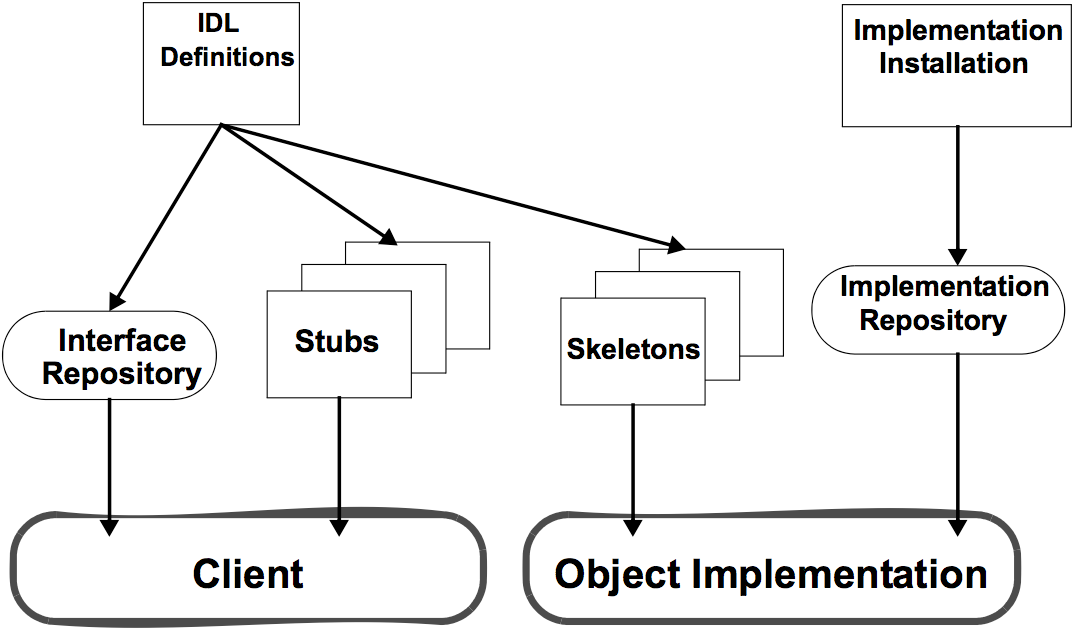
\includegraphics[width=\textwidth]{corba-client-object.png} %uncomment to enable image
    \caption{Interface and Implementation Repositories in CORBA, from \cite{isocorba}}
    \label{fig:corba-interfaces}
\end{figure}

TODO: Write more about CORBA using the CORBA paper. \cite{vinoski1997corba}


%---------------------------------------------------------------------------------------------------------------------%
% JSON-RPC and XML-RPC
%---------------------------------------------------------------------------------------------------------------------%
\subsection{JSON-RPC and XML-RPC}
XML-RPC is a simple RPC protocol which uses XML (Extended Mark-up Language) to define remote method calls and responses. It uses explicit data typing - the method name and parameters are hard-coded in the message itself. Messages are typically transported to remote servers over HTTP\footnote{Hyper-text transport protocol (HTTP) is the most common transfer protocol used by clients and servers to transfer data on the web}. Many implementations of XML-RPC exist in several different languages. 

For example, we could represent the RPC function call we defined before (Listing \ref{samplerpc}) as the XML-RPC function call shown in Listing \ref{examplexmlcall}.

\lstset{language=xml,caption={An example XML-RPC call},label=examplexmlcall}
\begin{lstlisting}
<methodCall>
  <methodName>
    generate_keypair
  </methodName>
  <params>
    <param><value><string> myPassPhraseHere </string></value></param>
  </params>
</methodCall>
\end{lstlisting}

The XML-RPC implementation could give a better interface for the XML calls. For example, run-time reflection APIs could be used to dynamically translate procedure calls into XML-RPC requests. The response from the server would also be in XML form. For example, the response for the request shown in Listing \ref{examplexmlcall} would be as shown in Listing \ref{examplexmlresponse}.

\lstset{language=xml,caption={An example XML-RPC response},label=examplexmlresponse}
\begin{lstlisting}
<methodResponse>
  <params>
    <param>
        <value>
          <struct>
            <member>
              <name>public_key</name>
              <value><string>qo96IJJfiPYWy3q3p5nvbNME87jG</string></value>
            </member>
            <member>
              <name>private_key</name>
              <value><string>IIEpAIBAAKCAQEA4eLvDruo9CswdW</string></value>
            </member>
          </struct>
        </value>
    </param>
  </params>
</methodResponse>
\end{lstlisting}

XML-RPC supports simple types like integer, double, string, boolean values. It also supports some complex types like arrays, and associative arrays (\lstinline{struct}). An example of this is in Listing \ref{examplexmlresponse}, where our structure has two keys with their respective values. Binary data can be Base64\footnote{Base64 is an encoding scheme that represents binary data as an ASCII string} encoded and sent in a \lstinline{<base64 />} tag. Because of the fixed language, XML-RPC is naturally cross-language compatible, as it is up to the two ends (client and server) to implement and use their own XML parsers and converters. Several libraries in different languages exist that do this.

XML-RPC and JSON-RPC are very similar. JavaScript Object Notation (JSON) is a simple and light-weight human-readable message format. Its advantages over XML is that it is a lot lighter and simpler. However, XML can be extended to support complex user-defined types using XML-Schemas, which is not possible directly using JSON. JSON-RPC is also a protocol and message format, for which different implementations exist. For example, we can easily represent the RPC call and response shown in Listings \ref{examplexmlcall} and \ref{examplexmlresponse} using the JSON-RPC protocol format as shown in Listing \ref{examplejsonrpc}.
\\

\lstset{language=c,caption={An example JSON-RPC request and response},label=examplejsonrpc}
\begin{lstlisting}
// JSON-RPC request:
{ 
  "jsonrpc": "2.0", 
  "method": "generate_keypair", 
  "params": ["myPassPhraseHere"], 
  "id": 1
}


// JSON-RPC response:
{
  "jsonrpc": "2.0", 
  "result": {
    "public_key": "qo96IJJfiPYWy3q3p5nvbNME87jG",
    "private_key": "IIEpAIBAAKCAQEA4eLvDruo9CswdW"
  }, 
  "id": 1
}

\end{lstlisting}

Both XML-RPC and JSON-RPC have well-defined protocols \cite{jsonrpcspec}\cite{xmlrpcspec}, and are implemented in many different languages.

%---------------------------------------------------------------------------------------------------------------------%
% RPC using Protocol Buffers
%---------------------------------------------------------------------------------------------------------------------%
\subsection{RPC using Protocol Buffers}
// TODO, see \href{https://code.google.com/p/protobuf/wiki/ThirdPartyAddOns#RPC_Implementations}{RPC implementations using protocol buffers}.
